\chapter{El problema}

En este capítulo se detallará a grandes rasgos cómo funciona el simulador de fútbol y los problemas que hay que tener en cuenta a la hora de diseñar un equipo.

\section{Servidor}

Es un sistema que permite a dos equipos jugar un partido de fútbol. La comunicación entre el servidor y los clientes se realiza mediante UDP/IP. Cada cliente es un proceso separado y se comunica con el servidor mediante un puerto. Cada equipo puede tener hasta 12 clientes (10 jugadores, 1 portero y 1 coach).

Los jugadores envían peticiones al servidor indicando las acciones que quieren realizar (patear, girar, correr, etc) y el servidor recibe estos mensajes y actualiza el ambiente acorde a las acciones de todos los clientes. Adicionalmente, el servidor provee a los clientes de información sensorial.

Es importante recalcar que el servidor es un sistema en tiempo real que trabaja con intervalos de tiempo discretos (o ciclos). Cada ciclo tiene una duración específica, así que las acciones que necesitan ser ejecutadas en un determinado ciclo deben llegar al servidor en el intervalo de tiempo correcto. Así, un bajo desempeño en un jugador puede resultar en oportunidades de acción perdidas que al final pueden perjudicar al equipo en general.

\subsection{Reglas de juego}

\textbf{Kick-off}
Se da inicio al juego, puede ser al inicio del primer o segundo tiempo o después de un gol. Los jugadores deben estar en su lado del campo para que esto pueda ocurrir. Se da un tiempo para que los jugadores se teletransporten a su posición deseada.

\textbf{Gol}
Se anuncia a todos los jugadores que hubo un gol y se pasa al estado Kick-off.

\textbf{Fuera de juego}
Cuando el balón sale del campo de juego, el referee mueve el balón a la posición apropiada, una línea lateral, una esquina o el área de gol, dependiendo de por donde salga el balón.

\textbf{Offside}
Un jugador está en offside si:
\begin{itemize}
\item Está en la mitad rival del campo
\item Está más cerca al arco rival que al menos 2 defensas
\item Está más cerca al arco que la pelota
\item Está más cerca al balón que 2,5 metros
\end{itemize}

\textbf{Backpass}
Al igual que en los partidos de fútbol reales, el arquero no puede atrapar el balón con las manos si esté le ha sido pasado por un jugador de su propio equipo. Esto terminaría en un tiro libre.

\textbf{Faltas en tiro libre}
Al hacer un tiro libre, un jugador no puede pasarse el balón a si mismo. Esto resultaría en un tiro libre para el otro equipo.

\textbf{Muerte súbita}
Si al terminar los 2 tiempos hay un empate, el partido continúa hasta que uno de los dos equipos anote un gol, el equipo que lo logre será el ganador.


\subsection{Mensajes al cliente}

El servidor puede enviarle los siguientes mensajes a los clientes: Escuchar mensaje de otro jugador, Mirar y Sentir cuerpo.


\section{Cliente}

Hay un cliente independiente por cada jugador, que le envía peticiones al servidor para realizar acciones y para consultar el estado actual. Puede enviarle los siguientes mensajes al servidor: Atrapar, Cambiar vista, Correr, Patear, Teletransportarse, Decir mensaje, Sentir cuerpo, Pedir marcador, Girar y Girar cuello. Ya que la comunicación con el servidor es vía UDP/IP, el cliente puede estar implementado en cualquier lenguaje de programación.


\subsection{Mensajes entre los jugadores}

Cada jugador puede escuchar a lo mucho un mensaje de cada equipo por cada ciclo de simulación. Un jugador sólo puede oír los mensajes de jugadores cercanos (dentro de un radio definido en el servidor). Sin embargo todos los jugadores pueden escuchar los mensajes del referee.

Si llegan más mensajes de los que un jugador puede escuchar, se escoge uno aleatoriamente y el resto se descarta. Es importante notar que un jugador puede enviar y recibir un mensaje al mismo tiempo.

\subsection{Percepción del ambiente}

Los agentes perciben el ambiente mediante el sensor de visión, que contrario a lo que se podría pensar, no retorna imágenes, sino la información ya procesada de lo que hay en el campo de visión. Es decir, el servidor envía a los clientes una lista de los objetos que el cliente ve en el campo de juego, junto con su dirección y su distancia. Entre estos objetos pueden aparecer jugadores del mismo equipo o rivales, las porterías, el balón o banderines que son usados para la ubicación de los jugadores.

Es importante notar que los agentes no conocen su posición $(x, y)$ dentro del juego, sino que tienen que deducirla a partir de los banderines que hay en el campo tal como muestra la figura \ref{fig:flags}.


\begin{figure}[htb]
\centering
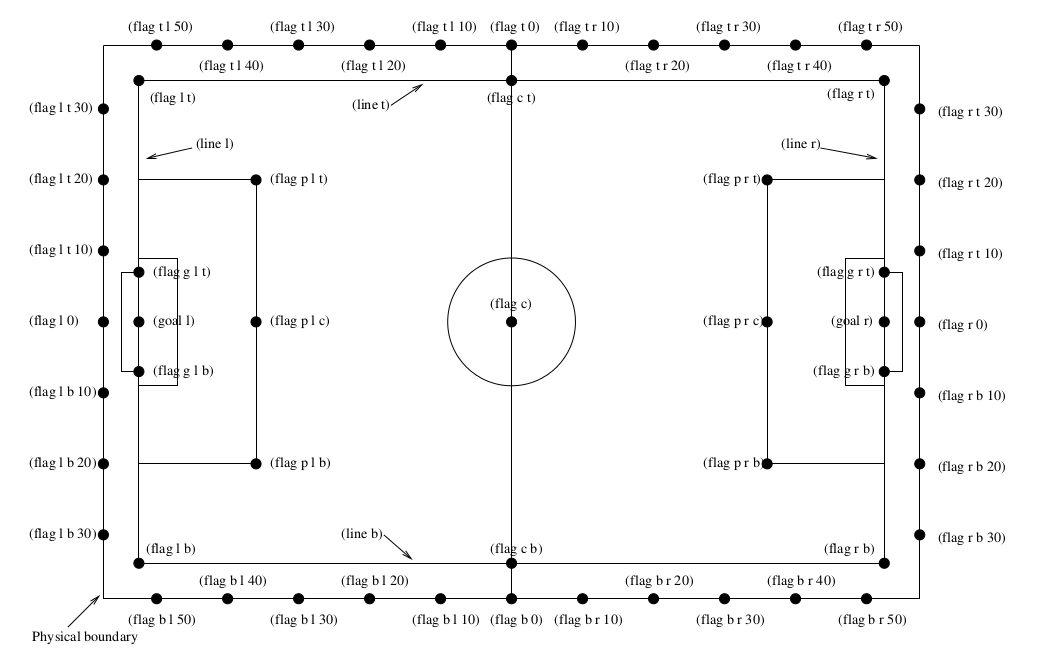
\includegraphics[width=150mm]{./graficos/flags.png}
\caption{Banderas en el campo de juego} \label{fig:flags}
\end{figure}

Además del sensor de visión, tenemos otro sensor de cuerpo que reporta el estado físico del jugador. Por ejemplo la estamina (necesaria para correr), la velocidad, el ángulo de la cabeza.


\section{Consideraciones finales}

En resumen, los problemas son que tenemos 11 agentes que deben jugar juntos con una capacidad limitada de comunicación. Que la representación del mundo, a pesar de ser de alto nivel, es muy compleja. Las acciones son continuas y además hay que controlar un gran número de parámetros que afectan cómo los agentes perciben el mundo. En los siguientes capítulos veremos conceptos que poco a poco nos llevarán a la resolución de este problema en la propuesta.